% !TEX program = xelatex
% AY2019 材料力学 解答例（同志社 生命医科学 医工学コース 院試）
% 問題・図は 01_exams/2019/tex を土台に、参考/ の粒度で解答を付した。
\documentclass[11pt,a4paper]{article}
\usepackage{../../00_common/preamble}
\usetikzlibrary{positioning,arrows.meta,calc,patterns,decorations.pathmorphing}

\title{材料力学 AY2019 解答例}
\author{}
\date{}

\begin{document}
\maketitle

\noindent\textbf{符号規約}：軸力・応力・伸びは引張りを正．たわみ $v$ は上向きを正，集中荷重 $W$ は下向きを正．
たわみの基礎式は $EI\,\dfrac{d^2v}{dx^2}=M(x)$ を用い，曲げモーメント $M$ は下に凸（さがり，サギング）を正とする．

%====================================================================
\section*{〔I〕}

図1に示すように $a$ および $c$ で固定された棒\textcircled{1}, 棒\textcircled{2}の接合点 $b$ に外力 $P$ が作用している.
この状態からさらに温度が $\Delta T$ 上昇した場合を考える. 各棒の初期長さを $L$, 断面積を $A$ とし,
$E$, $2E$ を縦弾性係数, $\alpha$, $2\alpha$ を線膨張係数とする. 次の問い (1) および (2) に答えよ.

\begin{center}
\begin{tikzpicture}[>=Latex]
  \fill[pattern=north east lines] (-0.5,-0.2) rectangle (0,2.2);
  \draw (0,-0.2) -- (0,2.2);
  \fill[pattern=north east lines] (9,-0.2) rectangle (9.5,2.2);
  \draw (9,-0.2) -- (9,2.2);
  \draw (0,0.4) -- (9,0.4);
  \draw (0,1.4) -- (9,1.4);
  \draw (4.5,0.4) -- (4.5,1.4);
  \draw[->,very thick] (4.5,0.9) -- (5.6,0.9) node[right]{$P$};
  \node[below] at (0,0.35) {a}; \node[below] at (4.5,0.35) {b}; \node[below] at (9,0.35) {c};
  \node at (2.2,0.95) {棒\textcircled{1}}; \node at (2.2,0.6) {\footnotesize $A,\,E,\,\alpha$};
  \node at (6.8,0.95) {棒\textcircled{2}}; \node at (6.8,0.6) {\footnotesize $A,\,2E,\,2\alpha$};
  \draw[<->] (0,1.75) -- (4.5,1.75) node[midway,fill=white]{$L$};
  \draw[<->] (4.5,1.75) -- (9,1.75) node[midway,fill=white]{$L$};
\end{tikzpicture}

\vspace{1mm}
図1
\end{center}

\begin{enumerate}[label=(\arabic*)]
  \item 棒\textcircled{1}と棒\textcircled{2}に生じる応力 $\sigma_1$, $\sigma_2$ を求めよ.
  \item 棒\textcircled{1}と棒\textcircled{2}の変位 $\lambda_1$, $\lambda_2$ を求めよ.
\end{enumerate}

\subsection*{解答}

\noindent\textbf{(1)}\quad 両端 $a,c$ が固定なので本問は不静定問題である．
接合点 $b$ の右向き変位を $u$（右向き正）とおき，これを未知数として変位法で解く．
各棒の軸力を $N_1,N_2$（引張り正），伸びを $\lambda_1,\lambda_2$ とする．

\medskip
\noindent\textit{適合条件（変位）}：棒\textcircled{1}は $a$ 端が固定で $b$ 端が $u$ だけ右に動くので，その伸びは $\lambda_1=u$．
棒\textcircled{2}は $b$ 端が $u$ だけ右に動き $c$ 端が固定なので，その伸びは $\lambda_2=-u$（縮む）．
各棒の伸びは「軸力によるもの＋温度によるもの」の和であるから
\[
  \lambda_1 = \frac{N_1 L}{EA} + \alpha L\,\Delta T = u,
  \qquad
  \lambda_2 = \frac{N_2 L}{2EA} + 2\alpha L\,\Delta T = -u .
\]

\noindent\textit{つり合い条件}：接合点 $b$ の水平方向のつり合い（右向き正）をとる．
棒\textcircled{1}は引張りなら $b$ を左へ $N_1$ で引き，棒\textcircled{2}は引張りなら $b$ を右へ $N_2$ で引くので
\[
  P - N_1 + N_2 = 0 \qquad\Longrightarrow\qquad N_1 - N_2 = P .
\]
上の 3 式から $u$ を消去すると
\[
  \frac{3EA}{L}\Big(u + \alpha L\,\Delta T\Big) = P
  \quad\Longrightarrow\quad
  u = \frac{PL}{3EA} - \alpha L\,\Delta T .
\]
これを軸力の式に戻すと
\[
  N_1 = \frac{P}{3} - 2EA\,\alpha\,\Delta T,
  \qquad
  N_2 = -\frac{2P}{3} - 2EA\,\alpha\,\Delta T .
\]
応力は $\sigma=N/A$ であるから
\[
  \ans{\;\sigma_1 = \frac{P}{3A} - 2E\alpha\,\Delta T,\qquad
        \sigma_2 = -\frac{2P}{3A} - 2E\alpha\,\Delta T\;}
\]
（$\sigma_2$ の負号は棒\textcircled{2}が圧縮側にあることを示す．）

\smallskip
検算：$N_1-N_2=\Big(\dfrac{P}{3}-2EA\alpha\Delta T\Big)-\Big(-\dfrac{2P}{3}-2EA\alpha\Delta T\Big)=P$ となり，
$b$ 点のつり合いを満たす ✓．

\medskip
\noindent\textbf{(2)}\quad (1) で求めた $u$ がそのまま棒\textcircled{1}の伸び $\lambda_1$，
その符号反転が棒\textcircled{2}の変形 $\lambda_2$ である．
\[
  \ans{\;\lambda_1 = u = \frac{PL}{3EA} - \alpha L\,\Delta T,\qquad
        \lambda_2 = -u = -\frac{PL}{3EA} + \alpha L\,\Delta T\;}
\]
$\lambda_1>0$ なら棒\textcircled{1}は伸び，$\lambda_2<0$ なら棒\textcircled{2}は縮む（$\Delta T$ の大小で符号は変わりうる）．

\smallskip
検算：両端固定で全長 $2L$ は不変だから，総変形は $\lambda_1+\lambda_2=0$ でなければならない．
実際 $\lambda_1+\lambda_2=u+(-u)=0$ となり適合する ✓．

%====================================================================
\clearpage
\section*{〔II〕}

長さ $2L$ の単純支持はりにおいて, はりの縦弾性係数を $E$, 断面 2 次モーメントを $I$ とした
場合に, 次の問い (1) および (2) に答えよ.

\begin{center}
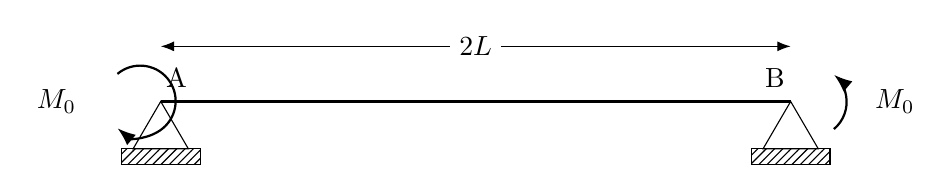
\begin{tikzpicture}[>=Latex]
  \draw[line width=1.2pt] (0,0) -- (8,0);
  \draw (0,0) -- (-0.35,-0.6) -- (0.35,-0.6) -- cycle;
  \draw[pattern=north east lines] (-0.5,-0.8) rectangle (0.5,-0.6);
  \draw (8,0) -- (7.65,-0.6) -- (8.35,-0.6) -- cycle;
  \draw[pattern=north east lines] (7.5,-0.8) rectangle (8.5,-0.6);
  \draw[->,thick] (-0.55,0.35) arc (130:-130:0.45);
  \node[left] at (-0.95,0) {$M_0$};
  \draw[->,thick] (8.55,-0.35) arc (-50:50:0.45);
  \node[right] at (8.95,0) {$M_0$};
  \node[above] at (0.2,0.05) {A}; \node[above] at (7.8,0.05) {B};
  \draw[<->] (0,0.7) -- (8,0.7) node[midway,fill=white]{$2L$};
\end{tikzpicture}

図2

\vspace{4mm}
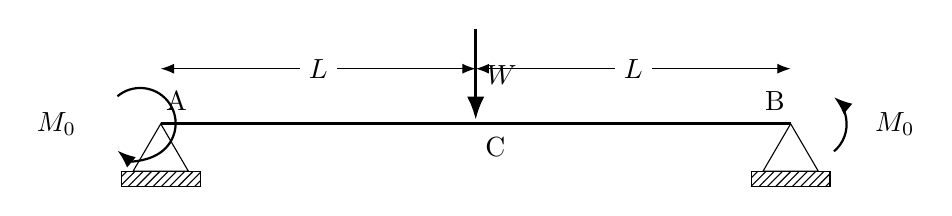
\begin{tikzpicture}[>=Latex]
  \draw[line width=1.2pt] (0,0) -- (8,0);
  \draw (0,0) -- (-0.35,-0.6) -- (0.35,-0.6) -- cycle;
  \draw[pattern=north east lines] (-0.5,-0.8) rectangle (0.5,-0.6);
  \draw (8,0) -- (7.65,-0.6) -- (8.35,-0.6) -- cycle;
  \draw[pattern=north east lines] (7.5,-0.8) rectangle (8.5,-0.6);
  \draw[->,thick] (-0.55,0.35) arc (130:-130:0.45);
  \node[left] at (-0.95,0) {$M_0$};
  \draw[->,thick] (8.55,-0.35) arc (-50:50:0.45);
  \node[right] at (8.95,0) {$M_0$};
  \draw[->,very thick] (4,1.2) -- (4,0.05) node[midway,right]{$W$};
  \node[above] at (0.2,0.05) {A}; \node[below right] at (4,-0.05) {C}; \node[above] at (7.8,0.05) {B};
  \draw[<->] (0,0.7) -- (4,0.7) node[midway,fill=white]{$L$};
  \draw[<->] (4,0.7) -- (8,0.7) node[midway,fill=white]{$L$};
\end{tikzpicture}

図3
\end{center}

\begin{enumerate}[label=(\arabic*)]
  \item 図2のように外力モーメント $M_0$ が両端 A と B に作用している場合を考える.
        はりのたわみ角とたわみの式を求めよ.
  \item 図3のように, 外力モーメント $M_0$ が両端 A と B に, 集中荷重 $W$ がはりの中央 C に
        負荷されている場合を考える. C でのたわみが 0 となる $W$ を求めよ.
\end{enumerate}

\subsection*{解答}

A 端を原点とし，はりに沿って右向きに座標 $x$（$0\le x\le 2L$）をとる．

\medskip
\noindent\textbf{(1)}\quad 両端に大きさ $M_0$ のモーメントが図2の向き（互いに逆回り）に作用するため，
両支点に鉛直反力は生じず（$R_A=R_B=0$），はり全長にわたって曲げモーメントの大きさは一定で $|M|=M_0$ となる．
図の向きのモーメントははりを上に凸（中央が持ち上がる）にたわませるので，
サギング正の規約では曲げモーメントは
\[
  M(x) = -M_0 \qquad (0\le x\le 2L)
\]
で一定である．基礎式 $EI\,v''=M(x)=-M_0$ を 2 回積分すると
\[
  EI\,v' = -M_0\,x + C_1,\qquad
  EI\,v  = -\frac{M_0}{2}x^2 + C_1 x + C_2 .
\]
両端単純支持の境界条件 $v(0)=0,\ v(2L)=0$ より
\[
  C_2 = 0,\qquad C_1 = M_0 L .
\]
よってたわみ角 $\theta(=v')$ とたわみ $v$ は
\[
  \ans{\;EI\,\theta(x) = M_0\,(L-x),\qquad
        EI\,v(x) = \frac{M_0}{2}\big(2Lx - x^2\big)\;}
\]
端でのたわみ角は $\theta_A=v'(0)=\dfrac{M_0 L}{EI}$，$\theta_B=v'(2L)=-\dfrac{M_0 L}{EI}$，
中央 C（$x=L$）のたわみは
\[
  v_C^{(M_0)} = v(L) = \frac{M_0}{2EI}\big(2L\cdot L - L^2\big) = \frac{M_0 L^2}{2EI}\quad(\text{上向き}).
\]

\smallskip
検算：$v(0)=0$，$v(2L)=\dfrac{M_0}{2EI}(4L^2-4L^2)=0$ で両支点のたわみが 0．
また $v'(L)=0$ となり，たわみは中央 $x=L$ について左右対称で，そこが最大（上向き）となる ✓．

\medskip
\noindent\textbf{(2)}\quad 重ね合わせを用いる．C 点のたわみは「両端モーメント $M_0$ による分」と
「中央集中荷重 $W$ による分」の和である．
(1) より前者は上向きに
\[
  v_C^{(M_0)} = \frac{M_0 L^2}{2EI}\quad(>0).
\]
スパン $2L$ の単純支持はり中央に下向き集中荷重 $W$ が作用するときの中央たわみは，
公式 $\dfrac{W\ell^3}{48EI}$（$\ell=2L$）より下向きに $\dfrac{W(2L)^3}{48EI}=\dfrac{WL^3}{6EI}$，すなわち
\[
  v_C^{(W)} = -\frac{WL^3}{6EI}\quad(<0,\ \text{下向き}).
\]
C 点のたわみが 0 となる条件 $v_C^{(M_0)}+v_C^{(W)}=0$ より
\[
  \frac{M_0 L^2}{2EI} - \frac{WL^3}{6EI} = 0
  \quad\Longrightarrow\quad
  W = \frac{3M_0}{L}.
\]
\[
  \ans{\;W = \dfrac{3M_0}{L}\;}
\]

\smallskip
検算：$W=\dfrac{3M_0}{L}$ を代入すると
$v_C^{(W)}=-\dfrac{1}{6EI}\cdot\dfrac{3M_0}{L}\cdot L^3=-\dfrac{M_0 L^2}{2EI}$ となり，
$v_C^{(M_0)}=+\dfrac{M_0 L^2}{2EI}$ とちょうど打ち消し合って $v_C=0$ となる ✓．

\end{document}
